% LaTeX layout by Jonas Kahler, jonas@derkahler.de
% HashTux SAD Document
% Group Tux:
% Aman Dirar, Jerker Ersare, Jonas Kahler, Dennis Karlberg
% Niklas le Comte, Marco Trifance, Ivo Vryashkov
% Chapter 6 - Logical View
\hypertarget{logicalview}{
\chapter{Logical View}}
Here, we present sequence diagrams showing how different operations take place
in the \textit{HashTux} application. \newline
The first 4 sequence diagrams describe the flow for a search request (the make
search use case). For the sake of clarity we have made several diagrams,
focusing on different parts of the system.
\newpage
\begin{figure}[ht]
  \centering
  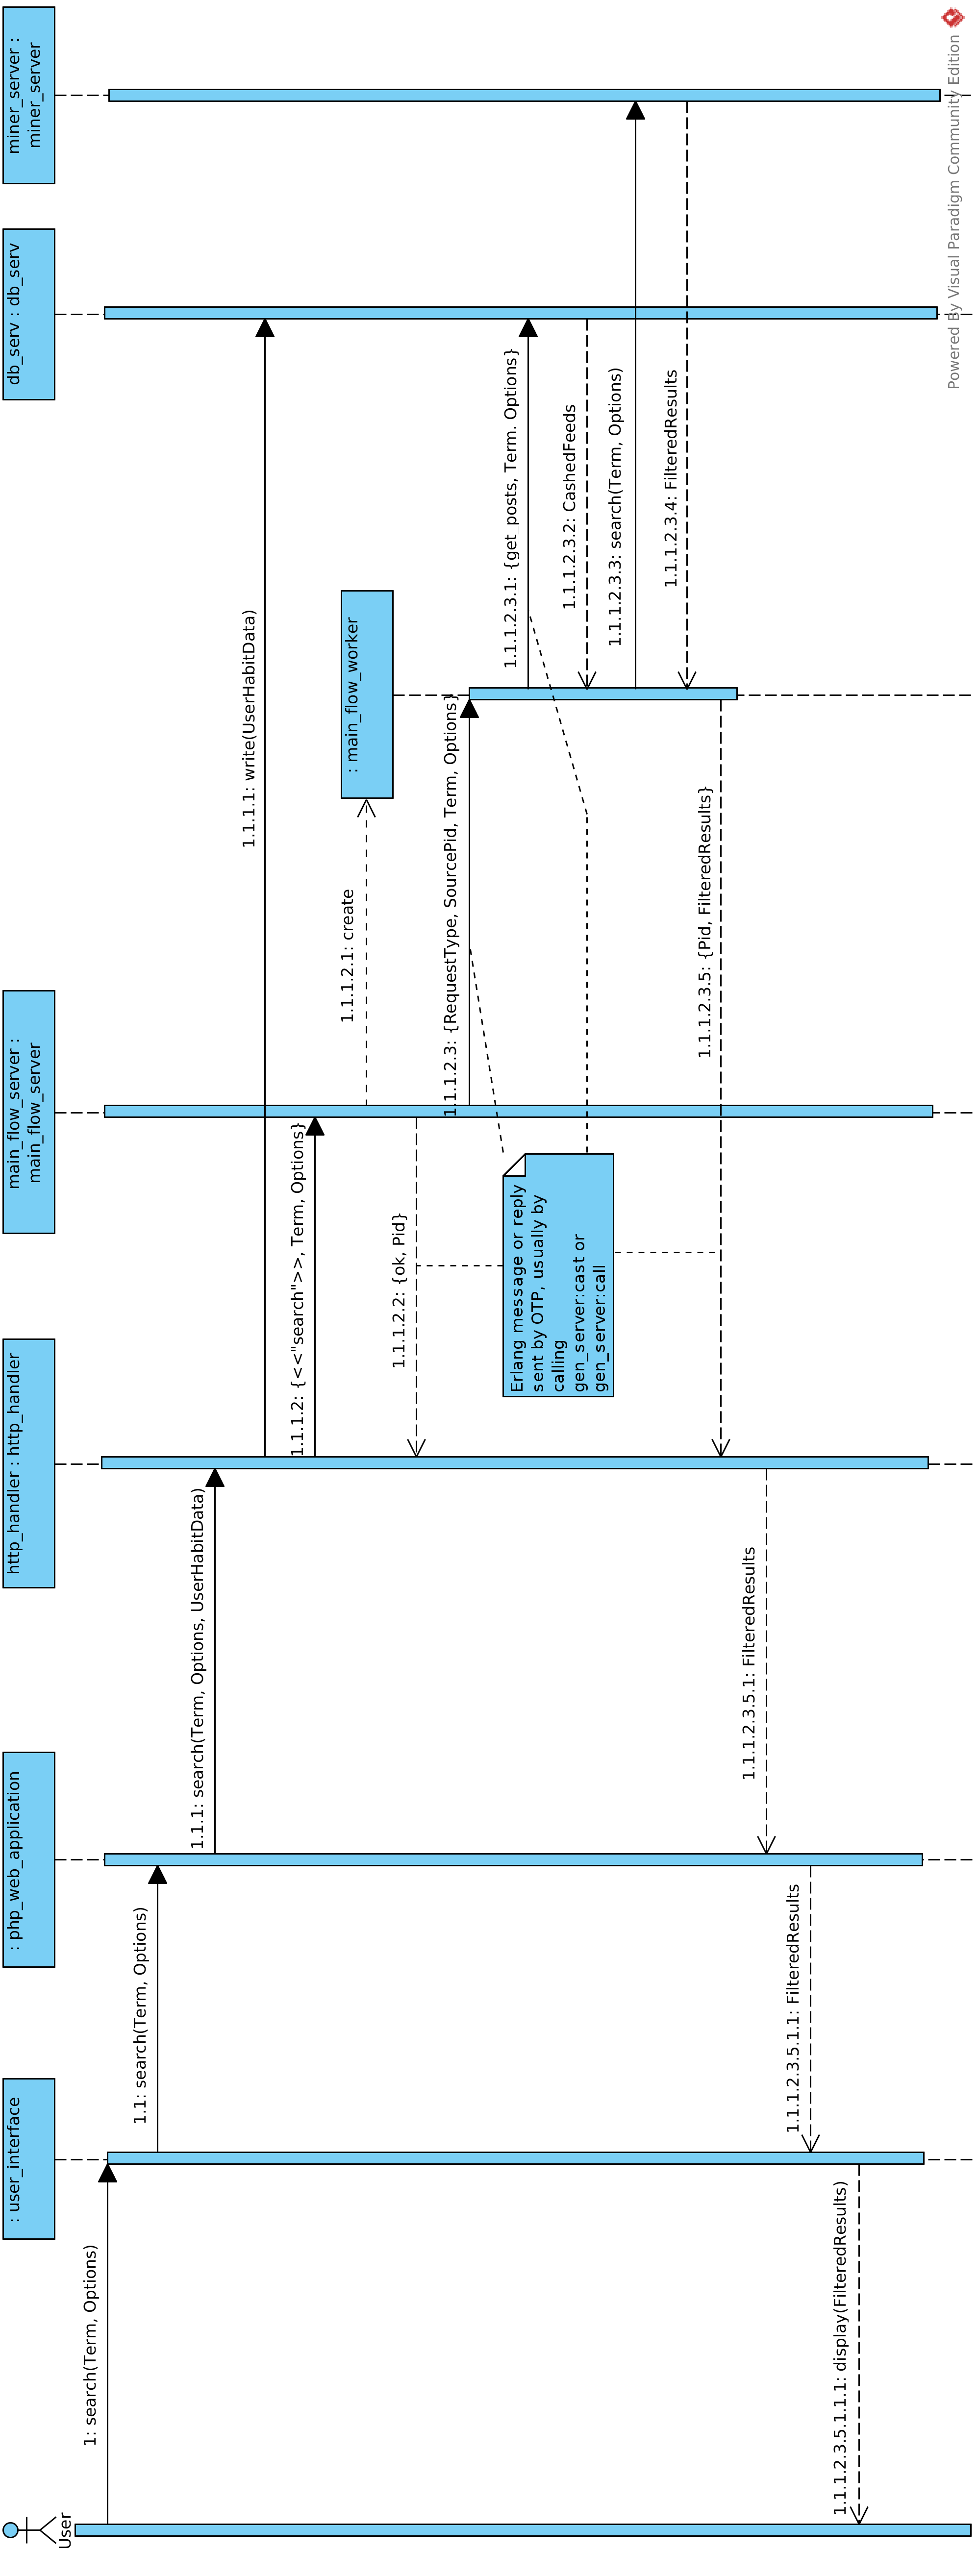
\includegraphics[width=0.6\textwidth]{search_request.png}
  \caption{Sequence of operations when a user executes a search}
\end{figure}
\newpage
\begin{figure}[ht]
  \centering
  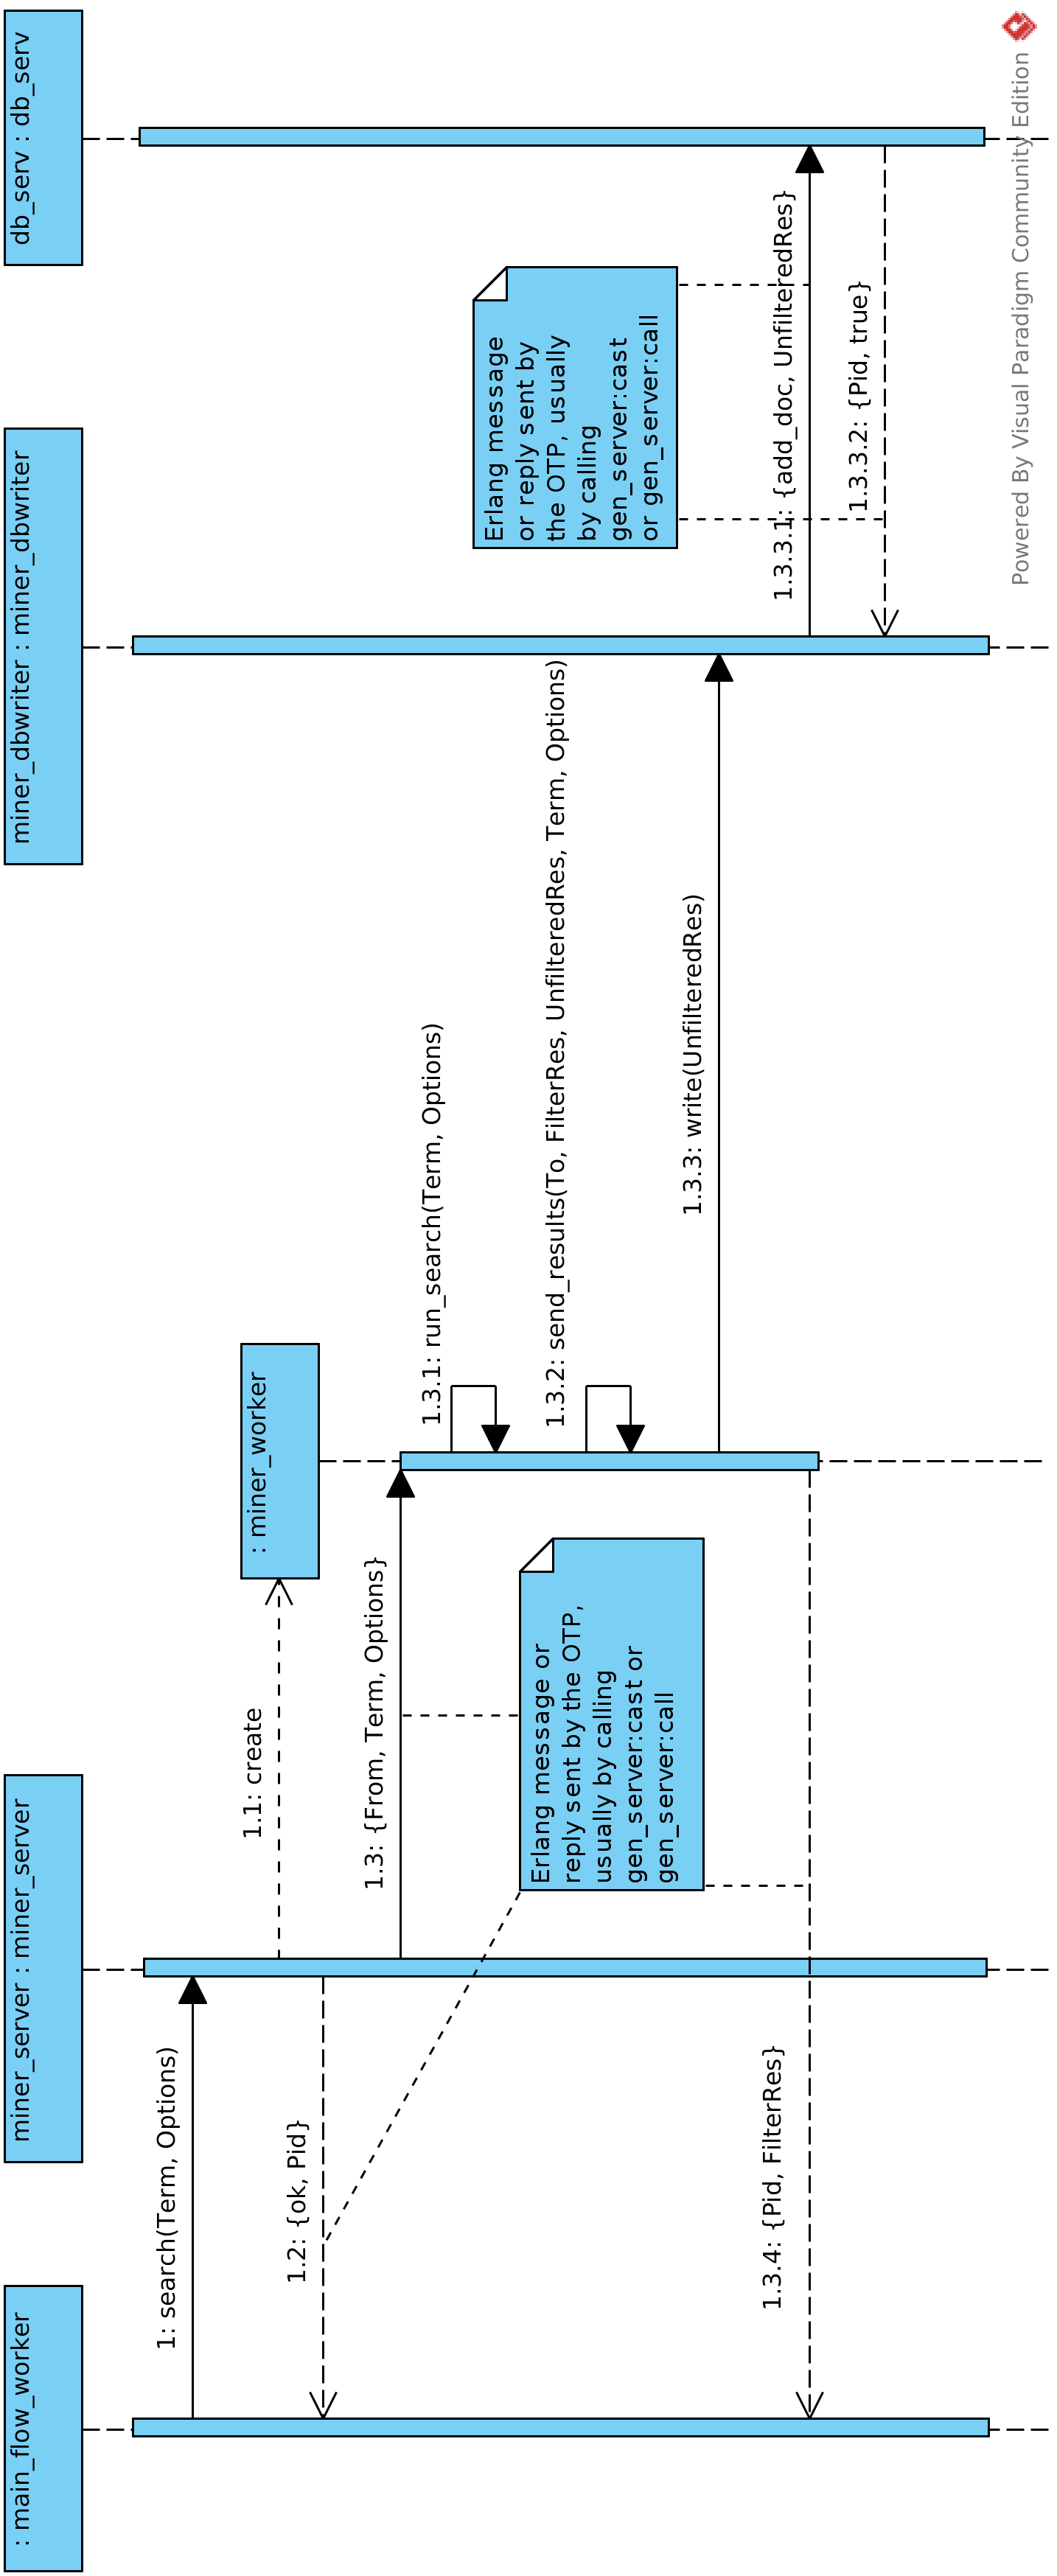
\includegraphics[width=0.62\textwidth]{miner_search.png}
  \caption{Sequence of operations when a search request is received in the miner
     server}
\end{figure}
\newpage
\begin{figure}[ht]
  \centering
  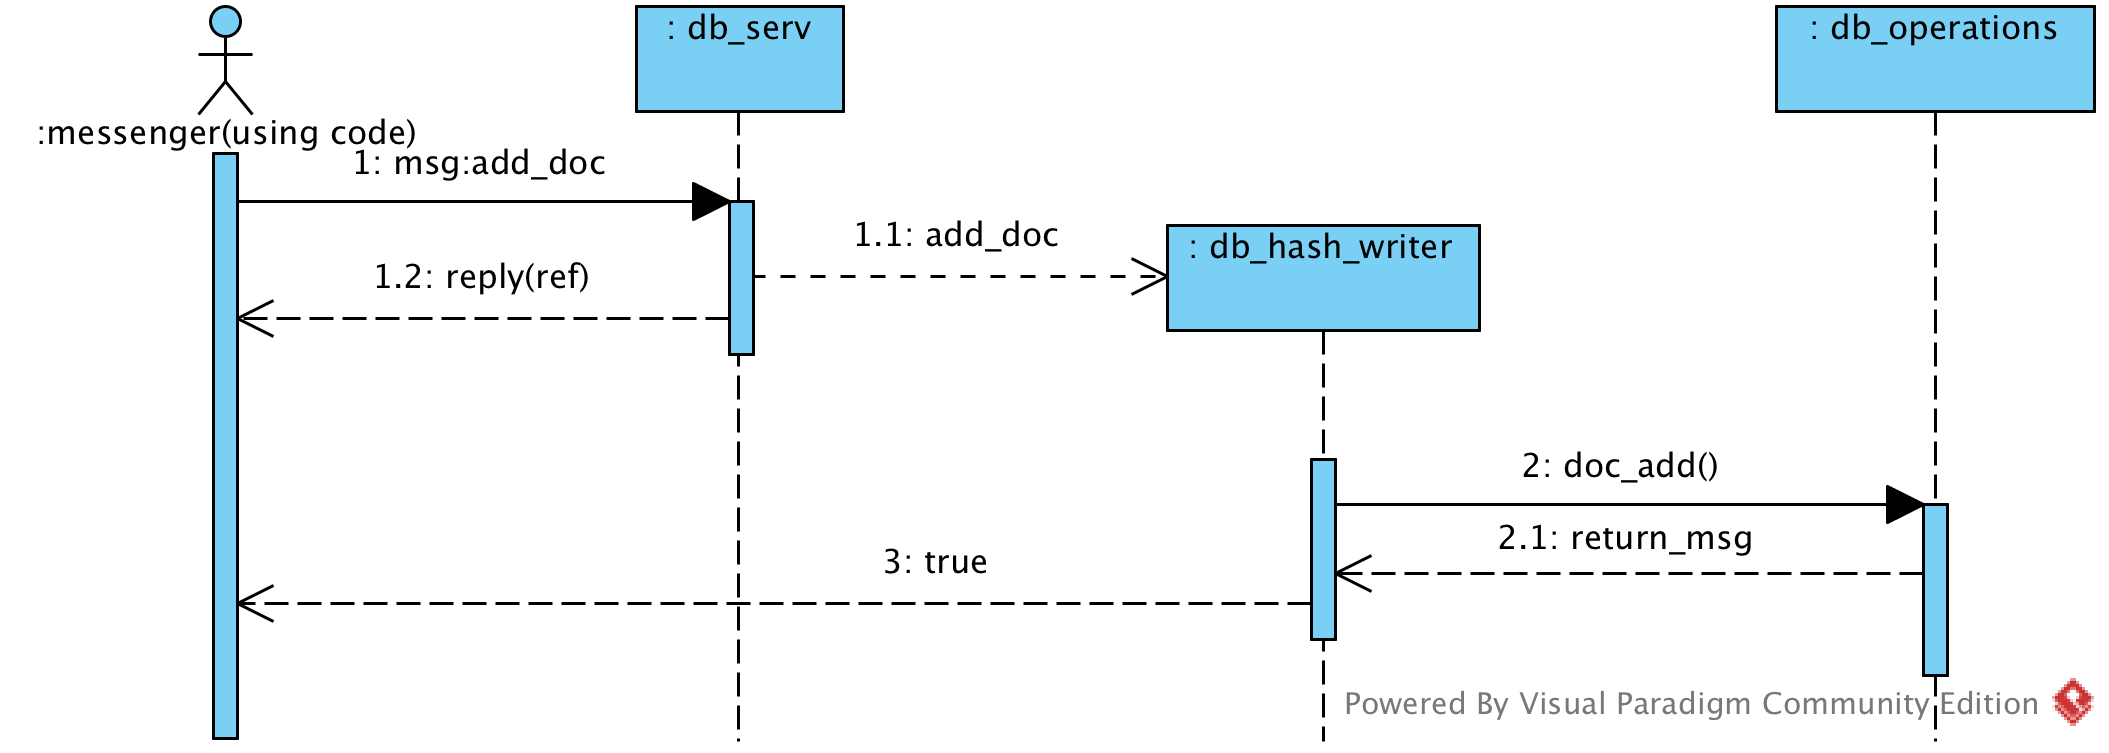
\includegraphics[width=1\textwidth]{write_to_hashtuxDB.png}
  \caption{This is the flow to write something to the HashTux database}
\end{figure}
\begin{figure}[ht]
  \centering
  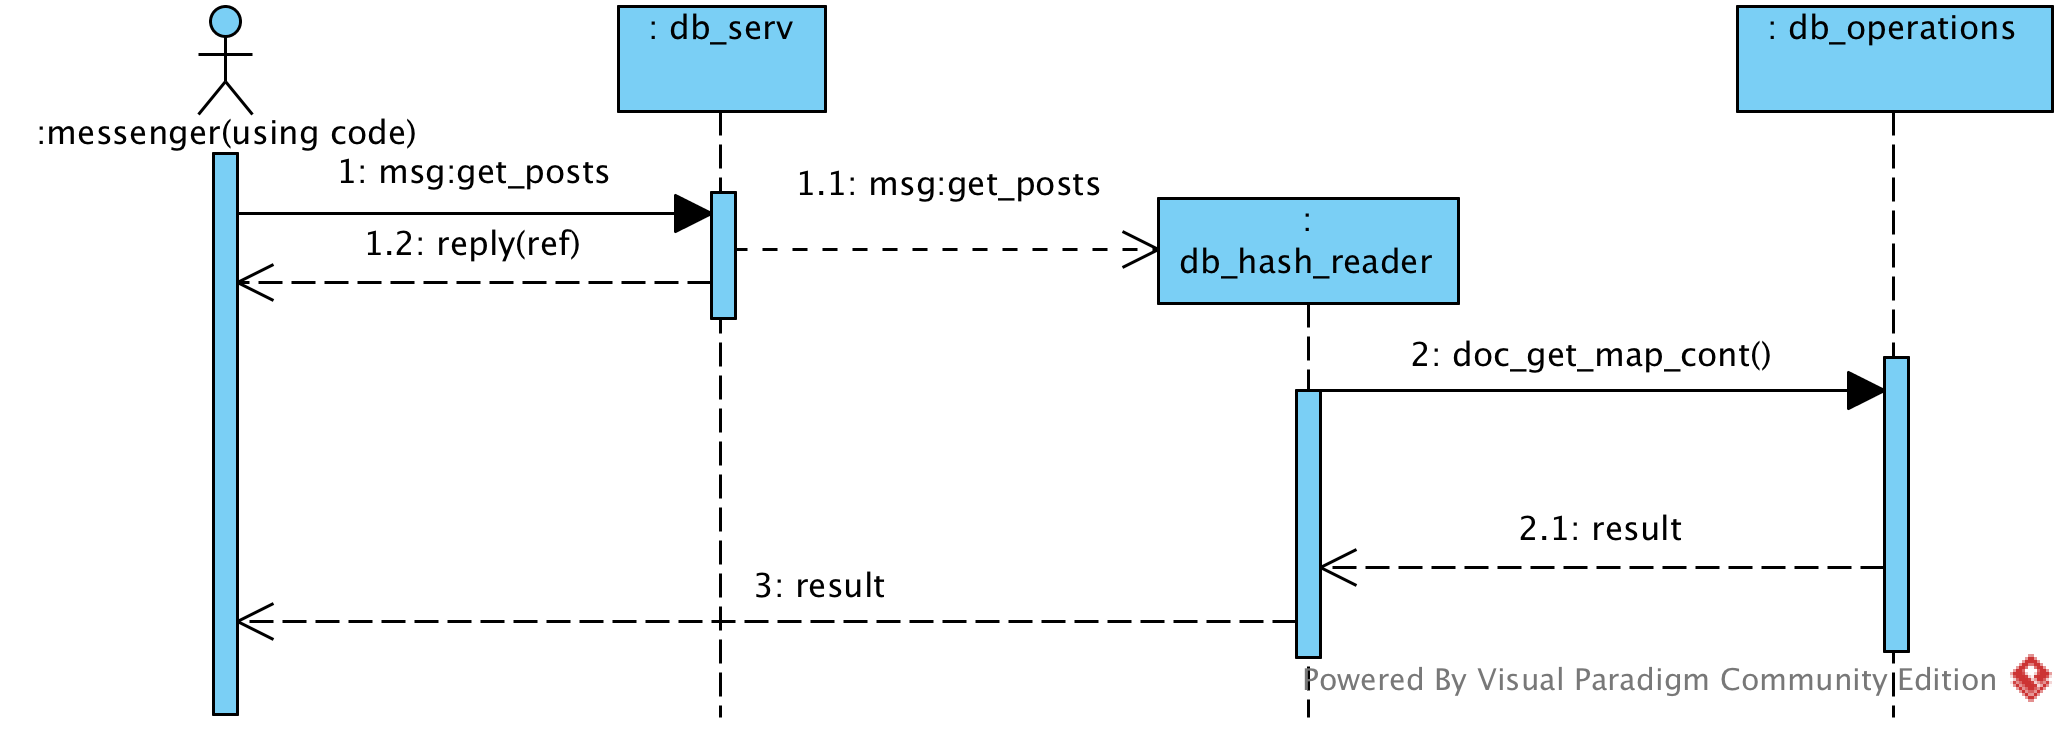
\includegraphics[width=1\textwidth]{read_from_hashtuxDB.png}
  \caption{This is the flow of reading the HashTux database to get results based
     on a search term}
\end{figure}
\begin{figure}[ht]
  \centering
  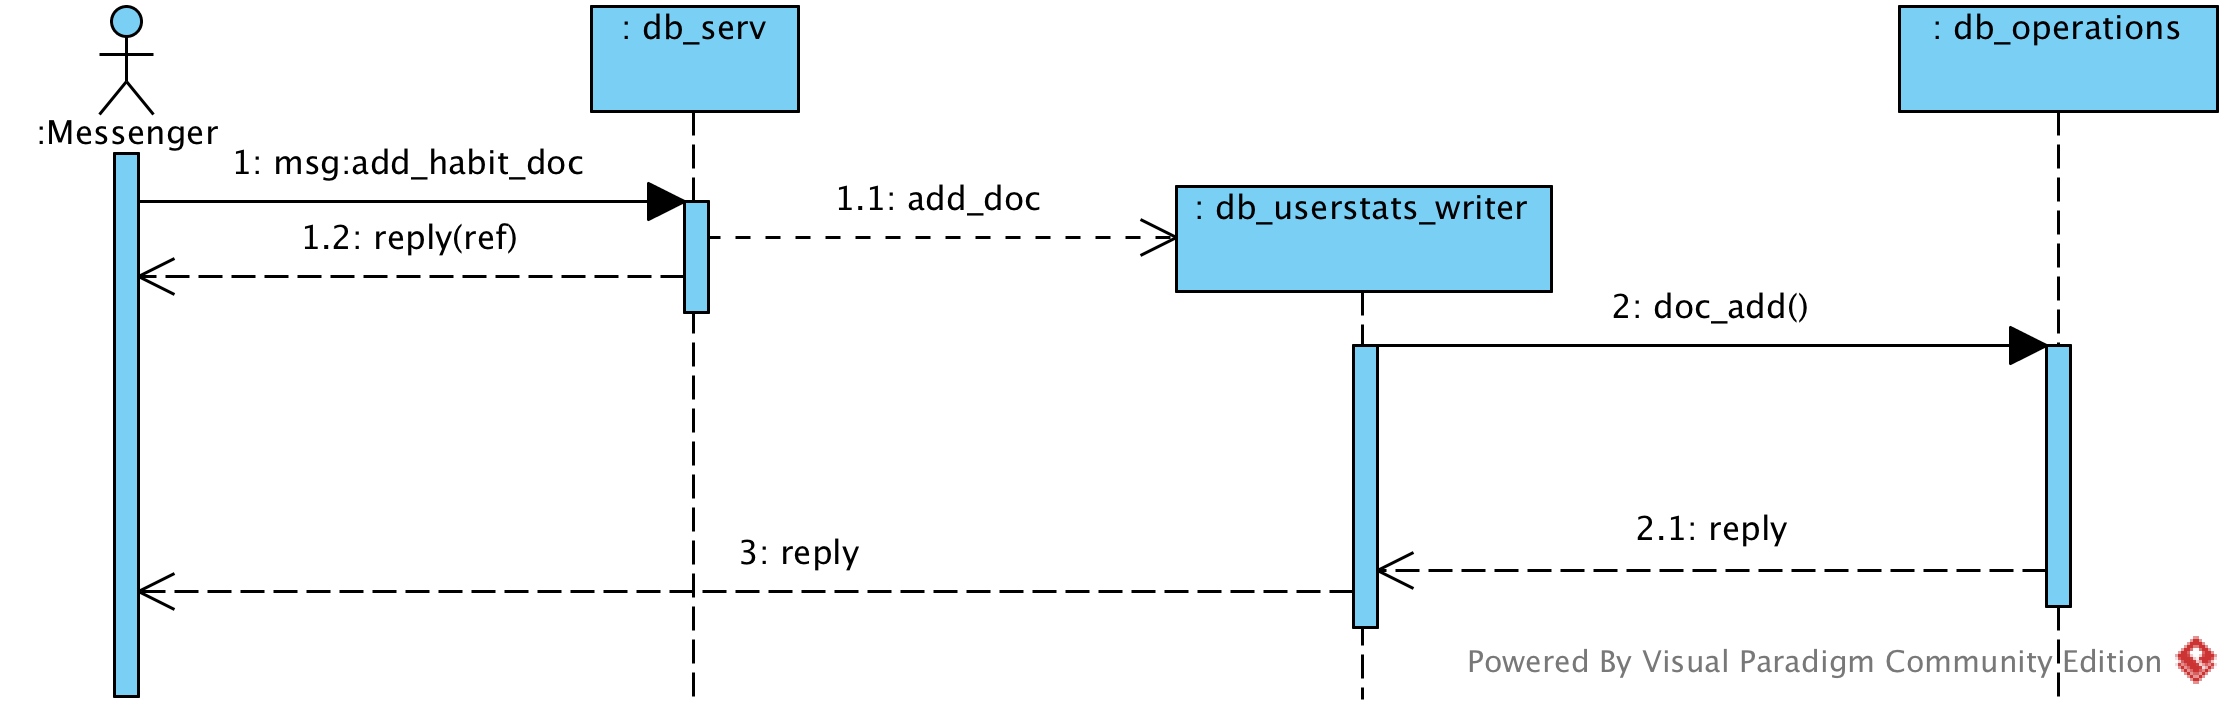
\includegraphics[width=1\textwidth]{write_to_hashtux_userstats.png}
  \caption{This is the flow to write something to the hashtux\textunderscore
     userstats database}
\end{figure}